\documentclass[letterpaper,10pt]{article}
\usepackage[top=2cm, bottom=1.5cm, left=1cm, right=1cm]{geometry}
\usepackage{amsmath, amssymb, amsthm, graphicx}
\usepackage{fancyhdr}
\pagestyle{fancy}

\lhead{\today}
\chead{Stat 440/640 Homework 1}
\rhead{Justin Hood}

\newcommand{\Z}{\mathbb{Z}}
\newcommand{\Q}{\mathbb{Q}}

\begin{document}
\begin{description}
\item[1.8]\hfill \\
We consider the following table,\\
\begin{center}
\begin{tabular}{ccc}
Year & PerCapita Income & Predicted Income \\\hline
1979 & 3074 & 3292 \\
1980 & 3135 & 3250 \\
1981 & 3206 & 3230 \\
1982 & 3267 & 3255 \\
1983 & 3310 & 3266 \\
1984 & 3362 & 3283 \\
1985 & 3418 & 3300 \\
1986 & 3500 & 3337
\end{tabular}
\end{center}
\begin{enumerate}
\item[a.] We use the equation,
\[e_i=y_t-\hat{y}_t\]
to compute the forecast error for each year. Thus,
\begin{center}
\begin{tabular}{cccc}
Year & PerCapita Income & Predicted Income & Forecast Error \\\hline
1979 & 3074 & 3292 & -218\\
1980 & 3135 & 3250 & -115\\
1981 & 3206 & 3230 & -24\\
1982 & 3267 & 3255 & 12\\
1983 & 3310 & 3266 & 44\\
1984 & 3362 & 3283 & 79\\
1985 & 3418 & 3300 & 118\\
1986 & 3500 & 3337 & 163
\end{tabular}
\end{center}
\item[b.] We then plot the error vs. time,
\begin{center}
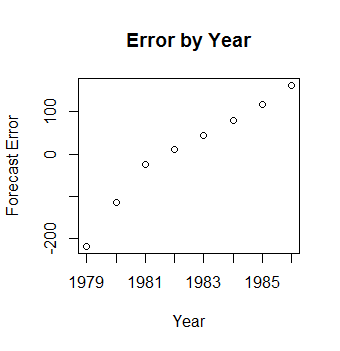
\includegraphics{errtime.png}
\end{center}
\item[c.] Based on the plot of error vs time, I do not think that this method adequately fits this data. Not only are the extreme values of error above 5\% of the true value, the error is not showing any signs of correcting towards the true value, indicating that the error could increase as the prediction is reported for later time values. It is worth noting, however, that the MAPE for this data is actually around 3\%, which is not as bad as the extremes.
\item[d.] We use the equation,
\[MAD=\frac{\sum_{t=1}^{n}|e_t|}{n}\]
to compute the MAD for the data. Thus,
\[MAD=\frac{773}{8}=96.625\]
\item[e.] We use the equation,
\[MSE=\frac{\sum_{t=1}^{n}(e_t)^2}{n}\]
to compute the MSE for the data. Thus,
\[MSE=\frac{110139}{8}=13767.375\]
\item[f.] We use the equation,
\[MAPE=\frac{\sum_{t=1}^{n}\frac{100|e_t|}{y_t}}{n}\]
to compute the MAPE for the data. Thus,
\[MAPE=\frac{23.6646}{8}\approx 2.9581\]
\end{enumerate}
\item[1.9]\hfill\\
We consider the following table,\\
\begin{center}
\begin{tabular}{cccc}
Year & Actual & Method A & Method B \\\hline
1998 & 8.0 & 9.0 & 9.5 \\
1999 & 12.0 & 11.5 & 10.5 \\
2000 & 14.0 & 14.0 & 12.0 \\
2001 & 16.0 & 16.5 & 13.0 \\
2002 & 10.0 & 19.0 & 15.0
\end{tabular}
\end{center}
\begin{enumerate}
\item[a,b] We now compute the MAD and MSE for each method as above.\\
\begin{center}
\begin{tabular}{ccc}
Method & MAD & MSE \\\hline
A & 2.2 & 16.5\\
B & 2.6 & 8.5
\end{tabular}
\end{center}
\item[c.] We note that these measures of forecast accuracy provide different values for each of the two methods. The difference in the MAD values is purely based upon the absolute errors, i.e. the method with predicted values closest to the true values will have a lower MAD score. The difference in the MSE values is computed as a function of squared error. Thus, we see that predicted values that are close to the true value are reduced, and values that are far from the true value are increased, resulting in a more significant difference in values.
\end{enumerate}
\item[2.2]\hfill\\
We consider the following dollar amounts,
\[\$99,\ \$123,\ \$75,\ \$138,\ \$105,\ \$65,\ \$116\]
\begin{enumerate}
\item[a.] We compute the sample mean, $\bar{y}$,
\[\bar{y}=\frac{\sum_{i=1}^n y_i}{n}=\frac{721}{3}=103\]
\item[b.] We then compute the sample variance, $s^2$,
\[s^2=\frac{\sum_{i=1}^{n}(y_i-\bar{y})^2}{n-1}=673.6667\]
\item[c.] Finally, we compute the sample standard deviation, $s$,
\[s=\sqrt{s^2}=25.95509\]
\end{enumerate}
\item[2.6]\hfill\\
We consider the table of ``Bag Weights" from the text book.\\
\begin{enumerate}
\item[a.] We compute the sample mean, $\bar{y}$,
\[\bar{y}=50.4333\]
\item[b.] We then compute the sample variance, $s^2$,
\[s^2=0.7880\]
\item[c.] We then compute the sample standard deviation, $s$,
\[s=0.88769\]
\item[d.] Below, a histogram of the data,
\begin{center}
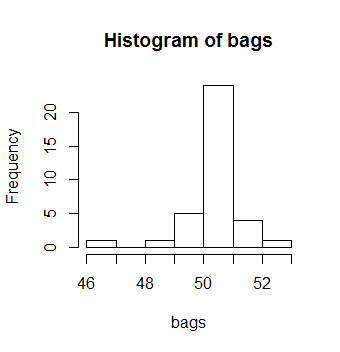
\includegraphics{bagshist.png}
\end{center}
\item[e.] Finally, we create a stem and leaf plot as follows,\\
\begin{verbatim}
  46 | 8
  47 | 
  48 | 
  49 | 018889
  50 | 122334455666666778888888
  51 | 124
  52 | 02
\end{verbatim}
\end{enumerate}
\end{description}


\end{document}
